\documentclass[11pt]{article}

% Generic, journal-agnostic preamble. Before submission, replace this with the
% official Overleaf/LaTeX template for the target journal and re-flow these
% sections into it -- the content is written to be template-independent.

\usepackage[utf8]{inputenc}
\usepackage[T1]{fontenc}
\usepackage{graphicx}
\usepackage{amsmath}
\usepackage{amssymb}
\usepackage{booktabs}
\usepackage{hyperref}
\usepackage{tikz}
\usetikzlibrary{positioning, arrows.meta, fit, backgrounds}
\usepackage[margin=1in]{geometry}
\usepackage{caption}

\title{QuantumCraft: An Open-Source Minecraft Mod to Teach Quantum Circuits using a Real Statevector Simulator}

\author{
Rodrigo Picos\\
\small Universitat de les Illes Balears
\and
Stavros G. Stavrinides\\
\small Democritus University of Thrace
\and
George Stavrinides\\
\small Democritus University of Thrace
\and
Ariadna Picos\\
\small Universitat de les Illes Balears
\and
Gerard Picos\\
\small Universitat de les Illes Balears
}

\date{}

\begin{document}
\maketitle

\begin{abstract}
This paper presents QuantumCraft, an open-source modification (``mod'') for the sandbox
game Minecraft that transforms the game world into a quantum-circuit laboratory. Players
place single-qubit gate blocks (Pauli~$X$/$Y$/$Z$, Hadamard, $S$, $T$) and multi-qubit
control/target marker blocks along up to three parallel ``qubit line'' rows, laid out
left to right in the same time-ordered convention used by a standard quantum-circuit
diagram, then read out the result with a handheld probe -- either an exact, ideal
readout of every basis state's probability, or a genuine collapsing Born-rule
measurement. In contrast to a scripted or purely illustrative stand-in for quantum
behavior, every amplitude, probability, and measurement outcome QuantumCraft displays is
produced by an actual complex-amplitude statevector simulator applying real unitary gate
matrices, the same representation used by general-purpose quantum-circuit simulators, up
to and including a genuine controlled-controlled-NOT (Toffoli) gate and Born-rule
probabilistic collapse. This paper describes why Minecraft's existing redstone subsystem,
despite its established role as an entry point into classical digital logic, does not by
itself extend to representing a qubit's superposition, the system's software
architecture, the statevector formulation underlying it, the pedagogical rationale for
embedding a correct simulator within a game environment rather than a dedicated
notebook-based tool, and the verification methodology employed during development. The
paper concludes with a discussion of current limitations and a roadmap for classroom
evaluation.
\end{abstract}

\section{Introduction}
\label{sec:introduction}

Teaching the basic behavior of quantum circuits is difficult in part because the underlying
phenomena -- a qubit existing in superposition rather than a definite 0 or 1, a measurement
irreversibly collapsing that superposition to a single classical outcome, two qubits becoming
entangled such that neither can be described independently of the other -- have no
counterpart at all in classical, everyday intuition, unlike an RC charging curve or a
mechanical oscillator, each of which at least resembles something a student has already
observed. The conventional response pairs the mathematics of complex amplitudes and unitary
matrices with a notebook-based simulator or an online circuit composer such as IBM's Quantum
Composer or Google's Cirq, in which a student drags gates onto a schematic timeline and reads
off a resulting statevector or histogram. These tools are effective and widely used, but each
presents the circuit as a two-dimensional diagram manipulated with a mouse, once removed from
the kind of first-person, spatial construction a sandbox game affords.

Sandbox games occupy a distinctive position relative to this approach. Minecraft in
particular has an established record as an informal STEM learning environment
(Section~\ref{sec:related-work}), in part because constructing something inside it requires
systems thinking comparable to an engineering task while remaining playful and low
stakes~\cite{nebel2016mining}. Minecraft's own redstone subsystem is already a widely used
entry point into classical digital logic, examined further in
Section~\ref{sec:minecraft-mechanics}. No equivalent exists, however, for \emph{quantum}
circuits within the base game: redstone signals are boolean and locally deterministic, with
no built-in notion of superposition, complex amplitude, or entanglement between distant
signals.

This paper describes QuantumCraft~\cite{picos2026quantumcraft}, a modification (``mod'') for
the Fabric mod loader, released as free and open-source software under the MIT license, that
adds a small, complete set of quantum-circuit components to Minecraft: a qubit-line block
establishing one of up to three parallel timeline rows, a single cyclable gate block offering
the Pauli~$X$, $Y$, $Z$, Hadamard, $S$, and $T$ gates, a pair of control and target marker
blocks that together represent a controlled-NOT or, with two controls, a Toffoli gate, and a
handheld probe reading out either the exact probability of every basis state or a genuine
collapsing measurement. Placing gate and marker blocks along a qubit line, left to right in
time order, constructs an actual quantum circuit within the game world; probing that circuit
runs a real complex-amplitude statevector simulator, applying the exact unitary matrix for
each placed gate in sequence, rather than a scripted approximation of what a quantum computer
would report. An entangled Bell state built this way genuinely has zero probability of
appearing in the $|01\rangle$ or $|10\rangle$ basis states, and repeated measurements of it
genuinely reproduce a 50/50 split between $|00\rangle$ and $|11\rangle$, in the same sense
that CircuitSimCraft's~\cite{picos2026circuitsimcraft} RC charging curve is a real solution to the
underlying differential equation rather than an animation tuned to look right.

The remainder of this paper is organized as follows. Section~\ref{sec:related-work}
situates QuantumCraft relative to existing quantum-circuit simulators, the foundational
quantum-computing literature, and the literature on Minecraft in education.
Section~\ref{sec:minecraft-mechanics} examines which of Minecraft's own construction
mechanics the mod builds upon, and why redstone's existing role as an entry point into
classical digital logic does not, by itself, extend to representing a qubit.
Section~\ref{sec:architecture} describes the mod's own software architecture, in particular
the algorithm used to translate a player's in-world gate placement into a quantum circuit.
Section~\ref{sec:quantum-simulator} describes the statevector simulator itself, including the
gate set, the general controlled-gate and Toffoli mechanisms, and Born-rule measurement.
Section~\ref{sec:pedagogy} discusses the pedagogical rationale underlying each design choice,
and Section~\ref{sec:experiments} gives five complete, reproducible worked circuits -- a
single-qubit superposition, a Bell state, a phase-kickback demonstration, a three-qubit GHZ
state, and a Toffoli-gate truth-table verification -- built directly into the same world,
with exact gate sequences and closed-form expected results for each.
Section~\ref{sec:validation} describes how the simulator was verified during development.
Section~\ref{sec:limitations} discusses current limitations and planned classroom
evaluation, and Section~\ref{sec:conclusion} concludes.

\section{Related Work}
\label{sec:related-work}

\subsection{Quantum computing: foundations and simulators}

The idea that a quantum-mechanical system could simulate physics more efficiently than a
classical computer originates with Feynman~\cite{feynman1982simulating}; Deutsch subsequently
formalized a universal quantum computer~\cite{deutsch1985quantum} and, with Jozsa, gave the
first explicit problem for which a quantum algorithm provably outperforms any classical
deterministic one~\cite{deutschjozsa1992rapid}, the same phase-kickback mechanism
Section~\ref{sec:experiments} demonstrates directly in-world. Shor's
factoring~\cite{shor1997polynomial} and Grover's search~\cite{grover1996fast} algorithms
established quantum computing's practical significance beyond foundational interest.
Nielsen and Chuang's textbook~\cite{nielsenchuang2010} is the standard reference for the
statevector formalism, gate set, and measurement postulate this mod implements directly
(Section~\ref{sec:quantum-simulator}). General-purpose software simulators such as Qiskit and
Cirq, and hardware-backed composers such as IBM's Quantum Composer, let a user assemble a
circuit from a gate palette and inspect the resulting statevector or measurement histogram;
QuantumCraft uses the same underlying representation -- a complex-amplitude vector evolved by
successive unitary matrix multiplication -- but embeds it in a three-dimensional, first-person,
block-based world rather than a schematic canvas, mirroring the relationship CircuitCraft
bears to SPICE-family circuit simulators~\cite{picos2026circuitcraft}.

\subsection{Entanglement and reversible logic}

Two multi-qubit phenomena central to this mod's worked experiments
(Section~\ref{sec:experiments}) have their own foundational literature. Bell's
theorem~\cite{bell1964epr} established that the correlations a pair of entangled qubits
exhibit cannot be reproduced by any local hidden-variable theory, the theoretical result the
Bell-state experiment in Section~\ref{sec:experiments} illustrates operationally rather than
by rederiving the inequality itself; Greenberger, Horne, and Zeilinger's three-qubit
generalization~\cite{ghz1989going} (the ``GHZ state'') sharpens the same point using perfect
rather than merely statistical correlations, and is the target state of this mod's
three-qubit worked experiment. Toffoli's reversible-computing
construction~\cite{toffoli1980reversible} showed that any classical boolean function can be
computed by a reversible (and hence, in particular, quantum-realizable) circuit built from a
single universal three-input gate bearing his name; this mod's Toffoli-gate experiment
(Section~\ref{sec:experiments}) verifies exactly that reversible-AND truth table directly
against a real statevector simulation.

\subsection{Minecraft in education}
\label{sec:minecraft-in-education}

The instructional value of games and simulations has been studied extensively in general: a
meta-analysis by Sitzmann~\cite{sitzmann2011meta} found simulation games to be more effective
for training self-efficacy and knowledge retention than comparison instructional methods
across a range of technical domains. Minecraft occupies a disproportionately large share of
that broader literature. Microsoft maintains and markets a dedicated, classroom-oriented
variant of the game, \emph{Minecraft: Education Edition}, an indication of how extensively the
game had already been adopted informally by educators prior to this commercial
productization. Nebel et al.'s review~\cite{nebel2016mining} surveys this literature broadly
and identifies Minecraft's principal appeal for education as the same property that makes it
appealing as a game: an open, constructive world in which a learner's own artifact, rather
than a worked example, is the object of study, closely matching Papert's constructionist
framing~\cite{papert1980mindstorms}, discussed further in Section~\ref{sec:pedagogy}.

Published case studies span a range of subjects well outside computer science. Bos et
al.~\cite{bos2014mathematics} describe using Minecraft to teach elementary-school mathematics
concepts through building tasks; Short's account~\cite{short2012teaching} covers the use of
the game to teach general science concepts in a secondary-school setting; and Cipollone et
al.~\cite{cipollone2014creative} present a case study of Minecraft used as an open-ended
creative tool. Callaghan's survey~\cite{callaghan2016investigating} identifies a theme common
to each of these studies: teachers report high engagement fairly consistently, whereas
rigorously measured gains in specific learning outcomes are reported less often, a caveat
also present in the general simulation-games literature~\cite{sitzmann2011meta} and one this
paper does not claim to have resolved for QuantumCraft specifically
(Section~\ref{sec:limitations}).

Within that broader literature, the subset closest to the present paper's subject concerns
Minecraft's native redstone subsystem, already a common entry point for teaching classical
digital logic: players build logic gates, adders, and working memory cells entirely from
in-game blocks, and Dezuanni et al.~\cite{dezuanni2015redstone} document children describing
and reasoning about redstone circuits in explicitly electrical language, notwithstanding that
the underlying mechanic is discrete and boolean rather than continuous or quantum-mechanical
(Section~\ref{sec:minecraft-mechanics} discusses redstone's mechanics in more depth). Very
recent work has begun to examine quantum computing specifically as a computer-science
education topic in its own right~\cite{seegerer2021quantum}, independent of any game-based
delivery mechanism. To the author's knowledge, QuantumCraft is the first Minecraft
modification to embed a real statevector quantum-circuit simulator, rather than approximating
quantum behavior with the game's existing discrete, classical redstone mechanics, or
presenting quantum concepts purely through a companion notebook alongside the game.

\section{Minecraft as a Construction Substrate}
\label{sec:minecraft-mechanics}

A central claim of this work is that building a quantum circuit inside Minecraft constitutes
a meaningfully different experience from assembling one in a schematic-based composer.
Substantiating that claim requires describing precisely what ``building'' means within
Minecraft itself, and identifying which of the game's own mechanics the mod reuses, extends,
or deliberately avoids.

\subsection{The voxel world and the timeline metaphor}

Minecraft's world is a three-dimensional grid of one-metre cubes, or \emph{blocks}; nearly
every action available to a player reduces to placing and removing blocks within this grid.
QuantumCraft maps a standard quantum-circuit diagram directly onto this grid: one qubit
occupies one row of qubit-line blocks running east, and a gate or marker block placed some
distance east of a qubit line's anchor represents an operation applied at that row's
corresponding time step, exactly as a gate drawn some distance along a horizontal wire in a
textbook circuit diagram represents an operation at that point in time. A two-qubit gate
such as CNOT is built from a pair of control and target marker blocks placed at the
\emph{same} east-offset on two different qubit rows, reproducing the vertical connecting line
a circuit diagram draws between a control dot and a target symbol, except that no physical
wire block is required between them: Section~\ref{sec:architecture} describes how the mod's
scanner recognizes this correlation purely from the two markers' shared time column, without
needing an explicit connector the way CircuitCraft's electrical topology
requires~\cite{picos2026circuitcraft}. This is a deliberate departure from CircuitCraft's own
graph/union--find topology model (in which any two mutually conductive faces are
electrically joined): a quantum circuit is conventionally drawn, taught, and reasoned about as
a fixed number of horizontal time-ordered lines, not as an arbitrary wiring graph, so the
in-world representation was chosen to match the diagram a student already encounters in a
textbook or lecture slide, rather than reusing CircuitCraft's own metaphor merely for
consistency between the two mods.

\subsection{Redstone: why it does not extend to qubits}

The base game already provides an entire circuit-like subsystem, redstone, built around
\emph{redstone dust} (a wire-like block carrying a signal), \emph{redstone torches} and other
sources, and a large family of blocks that read an incoming signal to trigger an effect. A
redstone signal is an integer strength from 0 to 15, propagated through a discrete
neighbor-notification event fired once per game tick; despite having no continuous quantity
(CircuitCraft's own paper discusses this same mechanic at greater length in the
classical-circuits context~\cite{picos2026circuitcraft}), redstone is widely used, both
informally and as a subject of academic interest~\cite{nebel2016mining}, as an entry point
into digital logic:
players construct logic gates, adders, and working memory cells entirely from redstone
components, and commonly describe and reason about redstone circuits in explicitly
electrical language~\cite{dezuanni2015redstone}. That established role, however, does not
extend to representing a qubit, and for a reason more fundamental than redstone's
already-discrete signal strength: a redstone signal, whatever its strength, is always a
single, locally determined, publicly readable integer, whereas a qubit's defining property is
that it exists in a superposition of two amplitudes that cannot both be read out at once, and
two qubits can become entangled such that neither one's state is even well defined
independently of the other. No quantization of a single scalar signal, however fine, can
represent a joint property that literally does not decompose into a value held separately by
each of two locations, which is precisely why QuantumCraft introduces an entirely new
representation (Section~\ref{sec:architecture}) rather than attempting to encode qubits into
redstone's existing signal-strength mechanic the way some ad hoc community techniques
approximate a continuous analog value with it.

\subsection{Block entities and on-demand execution}

Minecraft's modding interfaces expose the \emph{block entity} construct for a block that must
retain arbitrary mutable data, and, if the block type requests it, execute code once per game
tick. Every gate, qubit line, and control/target marker in this mod is implemented as a block
entity for the same reason CircuitCraft's components are~\cite{picos2026circuitcraft}: it is
the platform's existing mechanism for state tied to a specific position. Unlike
CircuitCraft, however, none of QuantumCraft's block entities register a per-tick callback at
all: a quantum circuit has no continuous transient to track between gate applications the way
a charging capacitor does, so there is nothing for a circuit to be doing between one probe use
and the next. A circuit is instead scanned and run once, on demand, exactly when a player
right-clicks the probe against a qubit line (Section~\ref{sec:architecture}), which is both
simpler to implement and a closer match to how a real quantum computer is actually used: a
circuit is prepared once and then executed as a single shot, not continuously re-evaluated in
the background.

\subsection{What the mod adds}

Given the preceding discussion, the mod's own contribution is a new, purpose-built spatial
notation for a quantum circuit -- qubit rows as parallel timelines, single-qubit gates as
blocks placed directly on those rows, and multi-qubit correlation expressed through shared
time-columns across rows rather than through any wired connection -- together with a
genuine statevector simulator to execute whatever circuit that notation describes
(Section~\ref{sec:quantum-simulator}). Redstone itself plays no role in this mod at all,
unlike in CircuitCraft, where it is reused deliberately for the one concept it is genuinely
well suited to represent (a boolean on/off switch); no comparably suitable role for redstone's
existing mechanics was identified for a quantum circuit, since even the mod's classical
special case (Section~\ref{sec:experiments}'s Toffoli-gate experiment) is more directly
expressed as boolean amplitudes at basis states $|0\rangle$ and $|1\rangle$ than through a
signal-strength integer.

\section{System Architecture}
\label{sec:architecture}

QuantumCraft is built on Fabric, the same modding toolchain CircuitSimCraft
uses~\cite{picos2026circuitsimcraft}. The codebase is organized into five packages, shown in
Figure~\ref{fig:architecture}: a simulator package with no dependency on any Minecraft class
at all, a pair of packages describing the in-world blocks and their per-block state, a
networking package that scans a player's placed blocks into a circuit and reports the result
back to the client, and a client-only package responsible for rendering the probe's result
heads-up display.

\begin{figure}[htbp]
\centering
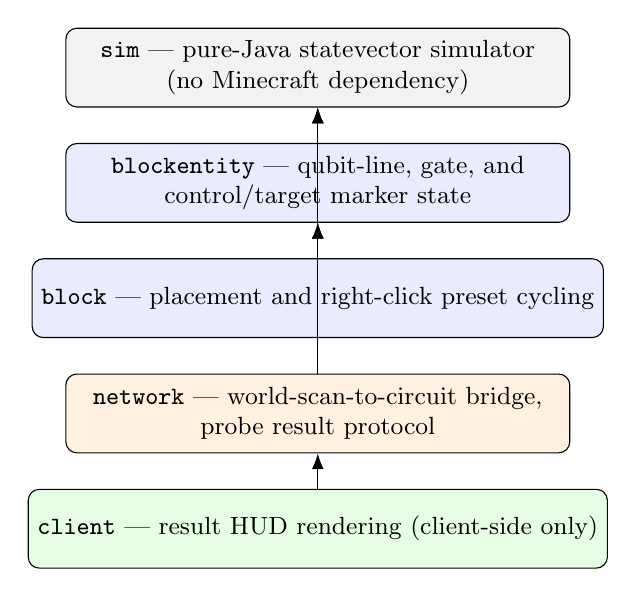
\begin{tikzpicture}[
    box/.style={draw, rounded corners, minimum width=6.4cm, minimum height=1cm,
                align=center, font=\small},
    node distance=0.45cm
]
\node[box, fill=gray!10] (sim) {\texttt{sim} --- pure-Java statevector simulator\\(no Minecraft dependency)};
\node[box, below=of sim, fill=blue!8] (blockentity) {\texttt{blockentity} --- qubit-line, gate, and\\control/target marker state};
\node[box, below=of blockentity, fill=blue!8] (block) {\texttt{block} --- placement and right-click preset cycling};
\node[box, below=of block, fill=orange!12] (network) {\texttt{network} --- world-scan-to-circuit bridge,\\probe result protocol};
\node[box, below=of network, fill=green!10] (client) {\texttt{client} --- result HUD rendering (client-side only)};

\draw[-{Latex[length=2mm]}] (blockentity) -- (sim);
\draw[-{Latex[length=2mm]}] (block) -- (blockentity);
\draw[-{Latex[length=2mm]}] (network) -- (blockentity);
\draw[-{Latex[length=2mm]}] (network) -- (sim);
\draw[-{Latex[length=2mm]}] (client) -- (network);
\end{tikzpicture}
\caption{Package-level architecture. As in CircuitSimCraft, the simulator has zero Minecraft
dependencies and is directly unit-testable with plain \texttt{javac}/\texttt{java}; every
other layer builds on it.}
\label{fig:architecture}
\end{figure}

\subsection{Qubit lines, gates, and markers}

A qubit-line block establishes one qubit's timeline row and carries no adjustable state of
its own. A single gate block, placed east of a qubit line's anchor, cycles through six
presets on right-click -- Pauli~$X$, $Y$, $Z$, Hadamard, $S$, and $T$ -- exactly as
CircuitSimCraft's diode cycles through its own preset family~\cite{picos2026circuitsimcraft}: one
block class serves every single-qubit gate rather than six separate block classes, keeping
the block/texture/recipe count tractable while still exposing the full single-qubit gate set
this mod supports. A control marker and a target marker, placed at the same east-offset on
two (for CNOT) or three (for Toffoli, with two control markers) different qubit rows,
together represent a multi-qubit gate; unlike every two-terminal component in
CircuitSimCraft, none of these blocks is directional, since a gate's effect does not depend on
which horizontal face a player was looking toward when it was placed.

\subsection{The world-scan-to-circuit bridge}

Unlike CircuitSimCraft's continuous, per-tick network rebuild, QuantumCraft constructs a circuit
only when a player right-clicks the probe against a qubit line, via a four-step scan.
First, a flood fill over six-face adjacency, following only positions whose block entity is a
qubit line, finds every qubit line connected to the clicked position. Second, the found lines
are sorted by position (their north--south coordinate primarily) to assign each a stable qubit
index from~0 up to the three-qubit cap this mod supports. Third, each qubit row is scanned
block by block to the east, up to a fixed maximum timeline length, recording whatever gate or
marker block entity, if any, occupies each offset. Fourth, the recorded entries are grouped by
their shared east-offset (their time column) and translated into circuit operations: a lone
gate entry becomes a single-qubit gate applied to its own row; one control marker paired with
one target marker at the same column becomes a controlled-NOT; two control markers paired
with one target becomes a Toffoli gate. Any other combination found within a single column --
an unpaired control with no target, two target markers, or more controls than the mod's
gate set supports -- is recorded as a warning and simply skipped rather than causing the scan
to fail, so an incompletely wired column fails safely, in the same spirit as CircuitSimCraft's
floating-node handling~\cite{picos2026circuitsimcraft}, rather than crashing or silently
misinterpreting the player's intent.

\subsection{The quantum probe}

A single handheld probe item right-clicked against a qubit line triggers the scan described
above, builds the resulting circuit's final statevector (Section~\ref{sec:quantum-simulator}),
and reports one of two things back to the clicking player, depending on whether the
interaction was a plain right-click or a shift-right-click. A plain right-click performs an
\emph{ideal readout}: every basis state's exact probability is computed and sent to the
client, with no randomness and no collapse, the same sense in which CircuitSimCraft's
oscilloscope displays an exact voltage rather than a noisy measurement. A shift-right-click
instead performs a genuine \emph{measurement}: the final statevector is sampled once, using
the standard Born-rule cumulative-probability procedure (Section~\ref{sec:quantum-simulator}),
the state is collapsed onto that single sampled outcome, and only that one classical outcome
-- not the full probability distribution that produced it -- is reported. This distinction is
made visually unmistakable in the result heads-up display (Figure~\ref{fig:hud}), which
labels the two modes ``IDEAL READOUT'' and ``MEASURED'' respectively and highlights only the
single collapsed row in the latter case, so that the difference between reading out amplitude
information no physical quantum computer could ever expose directly and performing an actual
one-shot measurement is never conflated.

\section{The Quantum Simulator}
\label{sec:quantum-simulator}

\subsection{Statevector representation}

The simulator follows the standard statevector formulation~\cite{nielsenchuang2010}. An
$n$-qubit register (QuantumCraft supports $n \in \{1,2,3\}$) is represented by a complex
amplitude vector $\psi \in \mathbb{C}^{2^n}$ indexed by basis state, using the little-endian
convention that qubit~0 is the least-significant bit of the index -- so, for two qubits, the
index ordering is $|00\rangle, |01\rangle, |10\rangle, |11\rangle$ with qubit~0 varying
fastest. A freshly constructed register is initialized to $\psi = (1, 0, \ldots, 0)$, the
all-zero basis state $|0\cdots0\rangle$, and every gate application below preserves the
invariant $\sum_i |\psi_i|^2 = 1$ by construction, since every matrix applied is unitary.

\subsection{Single-qubit gates}

A single-qubit gate is specified by a $2\times2$ unitary matrix; the mod exposes six presets,
each cycled by right-clicking a gate block (Section~\ref{sec:architecture}):
\begin{equation}
X = \begin{bmatrix} 0&1\\1&0 \end{bmatrix}, \quad
Y = \begin{bmatrix} 0&-i\\i&0 \end{bmatrix}, \quad
Z = \begin{bmatrix} 1&0\\0&-1 \end{bmatrix}, \quad
H = \frac{1}{\sqrt2}\begin{bmatrix} 1&1\\1&-1 \end{bmatrix}, \quad
S = \begin{bmatrix} 1&0\\0&i \end{bmatrix}, \quad
T = \begin{bmatrix} 1&0\\0&e^{i\pi/4} \end{bmatrix}.
\end{equation}
Applying such a matrix to qubit $q$ of an $n$-qubit register means: for every pair of basis
indices $(i, j)$ differing only in bit $q$ (with bit $q$ clear in $i$ and set in $j$), replace
$(\psi_i, \psi_j)$ with the matrix product of the $2\times2$ gate and the two-component vector
$(\psi_i, \psi_j)$, leaving every other amplitude untouched -- the direct implementation of
the tensor-product action $I \otimes \cdots \otimes U \otimes \cdots \otimes I$ without ever
materializing the full $2^n \times 2^n$ matrix.

\subsection{Controlled gates and the Toffoli}

A controlled-$U$ gate, of which CNOT ($U = X$) is the special case this mod's control/target
marker pair represents (Section~\ref{sec:architecture}), applies the single-qubit matrix $U$
to a target qubit only for those basis states in which a nominated control qubit's bit is~1,
leaving every basis state with the control bit clear entirely unchanged. This is implemented
as one general mechanism parameterized by an arbitrary $2\times2$ matrix, so a controlled-$X$
(CNOT), controlled-$Z$, or controlled-$Y$ all reduce to the same code path rather than three
separate implementations. The Toffoli gate (CCX), the doubly-controlled generalization
represented by two control markers and one target marker sharing a time column
(Section~\ref{sec:architecture}), applies the $X$ matrix's basis-flip only to those states in
which \emph{both} nominated control qubits' bits are~1: for every pair of basis indices
differing only in the target bit, with both control bits set in each, the two amplitudes are
swapped. Because a classical bit can be encoded as the basis state $|0\rangle$ or
$|1\rangle$ and never placed in superposition, the Toffoli gate applied to classical inputs
reproduces exactly the reversible-AND truth table Toffoli's own reversible-computing
construction describes~\cite{toffoli1980reversible}, verified directly in
Section~\ref{sec:validation} and demonstrated as a worked experiment in
Section~\ref{sec:experiments}.

\subsection{Measurement}

A measurement (triggered by a shift-right-click of the probe, Section~\ref{sec:architecture})
implements the standard Born rule~\cite{nielsenchuang2010}: a uniform random number in
$[0,1)$ is drawn and compared against the cumulative sum of $|\psi_i|^2$ over basis states in
index order, and the first index at which the cumulative sum exceeds the draw is the sampled
outcome. Every amplitude is then set to zero except the sampled outcome's, which is set to
$1$, collapsing the register exactly as an ideal projective measurement would. Because this
sampling procedure is only ever invoked once per probe use and the resulting register is
immediately discarded rather than persisted (Section~\ref{sec:architecture}), no mechanism is
needed to reset a register's state between uses, unlike a physical quantum computer or a
notebook-based simulator session, where explicit re-preparation between shots is often a
separate step.

\subsection{On-demand circuit execution}

A \texttt{QuantumCircuit} is simply an ordered list of operations -- single-qubit gates,
controlled gates, and Toffoli gates -- built directly from the world scan
(Section~\ref{sec:architecture}) rather than persisted as block-entity state anywhere. Running
a circuit allocates a fresh register initialized to $|0\cdots0\rangle$ and applies every
recorded operation to it in the scanned left-to-right (time) order, then discards the
intermediate register once a final result -- an ideal readout or a single measurement -- has
been reported to the player. There is, deliberately, no notion of a circuit's state persisting
between one probe use and the next: every probe use is a fresh, independent run of the whole
circuit from $|0\cdots0\rangle$, matching how a real quantum circuit is executed once as a
complete unit rather than incrementally advanced tick by tick the way CircuitCraft's
continuous MNA solve is~\cite{picos2026circuitcraft}.

\section{Pedagogical Design}
\label{sec:pedagogy}

Each design choice described in Sections~\ref{sec:architecture}
and~\ref{sec:quantum-simulator} was made with a specific misconception or missing intuition in
mind, in the spirit of Papert's constructionism~\cite{papert1980mindstorms}: a learner
constructs a working artifact and inspects its behavior directly, rather than observing that
behavior secondhand.

\textbf{Placing gates as physical blocks, not dragging icons onto a schematic.} A gate
occupies a specific block placed a specific number of steps east of a qubit line's anchor, and
right-clicking it cycles through its available presets in a fixed order. This arrangement is
closer to physically assembling an apparatus than to editing a diagram on a screen: a player
who wants to compare a Hadamard gate against a Pauli-$X$ gate must actually remove one block
and place (or cycle to) the other, in the same spirit that CircuitCraft asks a player to wire
and re-wire physical blocks rather than click a schematic's component library.

\textbf{An explicit distinction between an ideal readout and a real measurement.} A common
early misconception is treating ``the quantum state'' and ``what you measure'' as the same
thing, when the entire pedagogical point of measurement collapse is that they are not.
QuantumCraft's probe deliberately exposes both as separate, differently-labeled interactions
-- a plain right-click for the full, exact probability distribution (something no physical
quantum computer could ever hand a user directly), and a shift-right-click for a single,
collapsing, irreversible sample from that distribution -- so that a player must deliberately
choose which question to ask, rather than the mod quietly picking one on their behalf.
Figure~\ref{fig:hud} shows the resulting heads-up display for a Bell-state circuit
(Section~\ref{sec:exp-bell}) in each mode.

\begin{figure}[htbp]
\centering
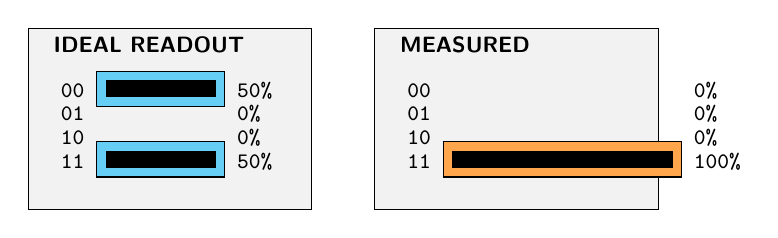
\begin{tikzpicture}[font=\footnotesize\ttfamily]
\begin{scope}
\node[draw, fill=gray!10, minimum width=3.6cm, minimum height=2.3cm, align=left, anchor=north west, inner sep=4pt] (idealbox) at (0,0) {};
\node[anchor=north west, font=\footnotesize\sffamily\bfseries] at (idealbox.north west) {\ \ IDEAL READOUT};
\node[anchor=north west] at ([yshift=-0.42cm]idealbox.north west) {\ \ 00\ \fcolorbox{black}{cyan!60}{\rule{1.4cm}{2.2mm}}\ 50\%};
\node[anchor=north west] at ([yshift=-0.72cm]idealbox.north west) {\ \ 01\ \phantom{\fcolorbox{black}{cyan!60}{\rule{1.4cm}{2.2mm}}}\ 0\%};
\node[anchor=north west] at ([yshift=-1.02cm]idealbox.north west) {\ \ 10\ \phantom{\fcolorbox{black}{cyan!60}{\rule{1.4cm}{2.2mm}}}\ 0\%};
\node[anchor=north west] at ([yshift=-1.32cm]idealbox.north west) {\ \ 11\ \fcolorbox{black}{cyan!60}{\rule{1.4cm}{2.2mm}}\ 50\%};
\end{scope}
\begin{scope}[xshift=4.4cm]
\node[draw, fill=gray!10, minimum width=3.6cm, minimum height=2.3cm, align=left, anchor=north west, inner sep=4pt] (measbox) at (0,0) {};
\node[anchor=north west, font=\footnotesize\sffamily\bfseries] at (measbox.north west) {\ \ MEASURED};
\node[anchor=north west] at ([yshift=-0.42cm]measbox.north west) {\ \ 00\ \phantom{\fcolorbox{black}{orange!70}{\rule{2.8cm}{2.2mm}}}\ 0\%};
\node[anchor=north west] at ([yshift=-0.72cm]measbox.north west) {\ \ 01\ \phantom{\fcolorbox{black}{orange!70}{\rule{2.8cm}{2.2mm}}}\ 0\%};
\node[anchor=north west] at ([yshift=-1.02cm]measbox.north west) {\ \ 10\ \phantom{\fcolorbox{black}{orange!70}{\rule{2.8cm}{2.2mm}}}\ 0\%};
\node[anchor=north west] at ([yshift=-1.32cm]measbox.north west) {\ \ 11\ \fcolorbox{black}{orange!70}{\rule{2.8cm}{2.2mm}}\ 100\%};
\end{scope}
\end{tikzpicture}
\caption{Schematic reconstruction of the probe's result heads-up display for the Bell-state
circuit of Section~\ref{sec:exp-bell}. Left: a plain right-click's ideal readout, showing the
exact 50/50 split between $|00\rangle$ and $|11\rangle$ with zero probability at
$|01\rangle$/$|10\rangle$. Right: a shift-right-click's measurement, collapsing to a single
sampled outcome (here $|11\rangle$) highlighted in a distinct color, with every other row at
0\%.}
\label{fig:hud}
\end{figure}

\textbf{A gate set small enough to reason about by hand, large enough to entangle and
interfere.} Six single-qubit presets and a two-marker multi-qubit mechanism are enough to
build every worked experiment in Section~\ref{sec:experiments} -- a superposition, an
entangled Bell pair, a phase-kickback interference effect, a three-qubit GHZ state, and a
Toffoli-gate truth table -- while remaining small enough that a student can, in principle,
multiply out every $2\times2$ or $4\times4$ matrix involved by hand and check the mod's
answer, the same verification discipline Section~\ref{sec:validation} itself uses. A larger
gate set (arbitrary rotation angles, for instance) was deliberately deferred
(Section~\ref{sec:limitations}) in favor of a fixed palette that keeps this hand-verifiability
intact.

\textbf{A hard cap of three qubits.} Restricting the register to at most three qubits keeps
every worked circuit's full $2^n$-dimensional statevector small enough to display every basis
state's probability at once in the result heads-up display (Figure~\ref{fig:hud}), rather than
requiring the player to scroll or select a subset of a much larger state space, while still
being large enough to demonstrate every multi-qubit phenomenon in this mod's scope: two
qubits are the minimum needed for entanglement at all, and three are the minimum needed for
both the Toffoli gate and a GHZ state.

\section{Worked Experiments}
\label{sec:experiments}

To ground the pedagogical claims of Section~\ref{sec:pedagogy} in something a reader can
reproduce rather than take on faith, this section specifies five complete circuits, each
built from the mod's own gate and marker blocks and each demonstrating a distinct piece of
standard introductory quantum-computing curriculum: a single-qubit superposition, a two-qubit
Bell state, a phase-kickback interference effect, a three-qubit GHZ state, and a
Toffoli-gate truth-table verification. Every circuit was built directly into the same
persistent world used throughout this paper's own development, laid out as five side-by-side
benches on a flattened platform beginning a few blocks east of the world's spawn point, so a
reader with access to that world can walk up to any of them immediately rather than
reconstruct them from a diagram.

\subsection{A methodological note on presets}

As with CircuitCraft's own components~\cite{picos2026circuitcraft}, no block entity in this
mod overrides Minecraft's block-entity NBT read/write methods, so every gate block, freshly
placed, loads at its hardcoded default preset (Pauli~$X$, the first entry in the cycle order
given in Section~\ref{sec:architecture}) regardless of which gate the experiment actually
calls for. Each experiment below states the exact number of right-clicks needed to reach the
intended gate, using the fixed cycle order
$X \to Y \to Z \to H \to S \to T \to X \to \cdots$. Because the default preset is already
$X$, a gate left completely unclicked functions as a bit-flip, which Experiment~\ref{sec:exp-toffoli}
below uses directly to prepare classical input states without needing any additional preset
at all.

\subsection{Experiment 1: single-qubit superposition}
\label{sec:exp-superposition}

The simplest circuit in this set: a single qubit line with one gate block placed one step
east of its anchor, right-clicked three times to cycle the gate from its default $X$ preset
to $H$ ($X \to Y \to Z \to H$). Built ten blocks east of spawn.

\textbf{Procedure.} Right-click the probe against the qubit line for an ideal readout.
Separately, shift-right-click it a few dozen times to accumulate a sample of individual
measurements.

\textbf{Expected result.} Starting from $|0\rangle$, the Hadamard gate produces
\begin{equation}
H|0\rangle = \frac{1}{\sqrt2}\left(|0\rangle + |1\rangle\right),
\end{equation}
so the ideal readout shows exactly 50\% at $|0\rangle$ and 50\% at $|1\rangle$, and repeated
measurements should show both outcomes appearing with roughly equal frequency, converging
toward that same 50/50 split as more shots are collected.

\subsection{Experiment 2: Bell state}
\label{sec:exp-bell}

Two parallel qubit lines (rows $q_0$ and $q_1$). A gate block on $q_0$, one step east of its
anchor, right-clicked three times to reach $H$, exactly as in
Experiment~\ref{sec:exp-superposition}. A control marker on $q_0$ and a target marker on
$q_1$, both two steps east of their respective anchors (the same time column), together
representing a CNOT with $q_0$ as control and $q_1$ as target. Built twenty blocks east of
spawn.

\textbf{Procedure.} Right-click the probe against either qubit line for an ideal readout (the
scan follows the shared qubit-line network regardless of which row is clicked,
Section~\ref{sec:architecture}).

\textbf{Expected result.} Starting from $|00\rangle$, the Hadamard produces
$\frac{1}{\sqrt2}(|00\rangle + |10\rangle)$ (recall qubit~0 is the least-significant, i.e.\
rightmost, digit), and the subsequent CNOT flips $q_1$ exactly when $q_0$ is~1, giving the
Bell state
\begin{equation}
\frac{1}{\sqrt2}\left(|00\rangle + |11\rangle\right),
\end{equation}
an exact 50\% at $|00\rangle$ and $|11\rangle$ and \emph{exactly zero}, not merely small, at
$|01\rangle$ and $|10\rangle$ -- the signature Bell's theorem shows cannot be reproduced by
two independently-behaving classical bits~\cite{bell1964epr}, reproduced here in Figure~\ref{fig:hud}'s
left panel. A shift-right-click measurement always yields either $00$ or $11$, never $01$ or
$10$, no matter how many times it is repeated.

\subsection{Experiment 3: phase kickback}
\label{sec:exp-kickback}

A single qubit line with three gates in sequence: $H$ one step east of the anchor (three
right-clicks, as above), $Z$ two steps east (two right-clicks, $X \to Y \to Z$), and a second
$H$ three steps east (three right-clicks again). Built thirty-four blocks east of spawn.

\textbf{Procedure.} Right-click the probe for an ideal readout.

\textbf{Expected result.} Although the qubit passes through an equal superposition twice, the
final state is a deterministic $|1\rangle$, not a 50/50 mixture:
\begin{equation}
H\,Z\,H\,|0\rangle = H\,Z\,\frac{1}{\sqrt2}(|0\rangle+|1\rangle)
= H\,\frac{1}{\sqrt2}(|0\rangle-|1\rangle) = |1\rangle,
\end{equation}
so the ideal readout shows exactly 0\% at $|0\rangle$ and 100\% at $|1\rangle$, and every
measurement returns $1$ with certainty. This is the same phase-kickback interference
mechanism that underlies the Deutsch--Jozsa
algorithm~\cite{deutschjozsa1992rapid}: information encoded purely in a relative phase (the
sign flip $Z$ applies to $|1\rangle$) becomes a deterministic, directly observable outcome
only once a second Hadamard converts that phase difference back into a population difference,
despite neither of the two intermediate superposition states individually revealing anything
about the sign at all.

\subsection{Experiment 4: three-qubit GHZ state}
\label{sec:exp-ghz}

Three parallel qubit lines ($q_0$, $q_1$, $q_2$). A gate block on $q_0$ one step east,
cycled to $H$ (three right-clicks). A control marker on $q_0$ and target marker on $q_1$, both
two steps east (CNOT, $q_0 \to q_1$). A second control marker on $q_0$ and target marker on
$q_2$, both three steps east (a second CNOT, $q_0 \to q_2$). Built forty-eight blocks east of
spawn.

\textbf{Procedure.} Right-click the probe against any of the three qubit lines for an ideal
readout.

\textbf{Expected result.} The Hadamard produces
$\frac{1}{\sqrt2}(|000\rangle + |100\rangle)$, and each subsequent CNOT copies $q_0$'s value
onto one more qubit, giving the three-qubit GHZ state~\cite{ghz1989going}
\begin{equation}
\frac{1}{\sqrt2}\left(|000\rangle + |111\rangle\right),
\end{equation}
an exact 50\% at $|000\rangle$ and $|111\rangle$ and exactly zero at every one of the
remaining six basis states -- perfect three-way correlation with no classical analogue, a
sharper demonstration of the same nonlocal correlation Experiment~\ref{sec:exp-bell}
illustrates with two qubits~\cite{ghz1989going}.

\subsection{Experiment 5: Toffoli gate as reversible AND}
\label{sec:exp-toffoli}

The most advanced circuit in this set, and the only one whose classical truth table is
checked exhaustively rather than read off a single run. Three parallel qubit lines ($q_0$,
$q_1$, $q_2$, the two controls and the target); a control marker on $q_0$ and a second control
marker on $q_1$, together with a target marker on $q_2$, all at the same time column, two steps
east of their respective anchors, leaving the one-step column free for the preparation gates
described next. Built sixty-four blocks east of spawn.

\textbf{Procedure.} The two control qubits' classical input is set by placing (or removing) a
gate block one step east of the anchor -- \emph{before} the Toffoli's own column, two steps
east -- on the corresponding row: leaving that position empty prepares that control as
$|0\rangle$ (the identity, i.e.\ no gate at all), while placing a freshly placed gate block
there -- its default preset, $X$, requiring zero right-clicks -- prepares that control as
$|1\rangle$. Repeat the shift-right-click
measurement once for each of the four combinations of the two controls' preparation gates
being present or absent, recording the target qubit's measured outcome each time; the target
line itself is left completely unprepared ($|0\rangle$) before every run.

\textbf{Expected result.} A Toffoli gate flips its target exactly when both controls are
$|1\rangle$, and leaves classical basis states as basis states (no superposition is ever
introduced by this circuit, since no Hadamard is used), so the four runs reproduce exactly the
reversible-AND truth table~\cite{toffoli1980reversible}
\begin{equation}
(c_1, c_2, t) \mapsto (c_1, c_2, t \oplus (c_1 \wedge c_2)),
\end{equation}
with $t=0$ throughout: $(0,0)\to$ target measures $0$; $(0,1)\to$ target measures $0$;
$(1,0)\to$ target measures $0$; $(1,1)\to$ target measures $1$, the one input combination for
which both controls are set. Every one of the four measurements returns its predicted outcome
with certainty (probability $100\%$ at that one basis state on the corresponding ideal
readout, $0\%$ everywhere else), since every input to this circuit is a classical basis state
rather than a superposition, illustrating concretely that a quantum computer's gate set is a
strict superset of classical reversible logic, not a wholly separate, unrelated formalism.

\section{Verification Methodology}
\label{sec:validation}

Because the central premise of the mod is that its behavior is not a scripted
approximation, the simulator was checked during development against nine closed-form and
statistical properties, each executable as a plain Java program requiring no game instance
(the \texttt{sim} package has no dependency on any Minecraft class at all, exactly as
CircuitCraft's solver package does~\cite{picos2026circuitcraft}): that $X|0\rangle$ produces
exactly $|1\rangle$; that a Hadamard applied to $|0\rangle$ produces exactly a 50/50
superposition; that the two-qubit Bell-state and three-qubit GHZ-state circuits of
Section~\ref{sec:experiments} produce their exact expected amplitudes; that a Toffoli gate
reproduces the reversible-AND truth table for all eight classical three-bit inputs; that the
phase-kickback circuit of Section~\ref{sec:exp-kickback} produces a deterministic $|1\rangle$;
that 20{,}000 simulated measurements of a Bell state never once produced a $|01\rangle$ or
$|10\rangle$ outcome and converged to within half a percentage point of the predicted 50\%
split; and that total probability remains exactly $1$ after a long sequence of mixed single-
and multi-qubit gates, confirming that every gate application preserves unitarity. All nine
checks passed.

Because the mod targets a version of Minecraft (26.2) released after the training data
cutoff of the large language model used to assist in its development, and because that
version introduced several breaking changes to modding-relevant application programming
interfaces, every such interface used by the \texttt{block}, \texttt{blockentity}, and
\texttt{network} packages (block registration, the two-phase heads-up-display rendering
interface, and the per-item model-definition file format) was checked directly against the
decompiled game source for this specific version prior to being relied upon, following the
same methodological practice established during CircuitCraft's own
development~\cite{picos2026circuitcraft}: verifying an assumption against the authoritative
source for the exact version in use, rather than against generic recollection of how
equivalent interfaces behaved in earlier versions of the game.

For transparency, it should be noted that, at the time of writing, the nine checks described
above were performed ad hoc during development rather than captured as a persisted,
automatically re-run test suite within the repository -- the same caveat, and the same
remedy, noted in CircuitCraft's own validation section~\cite{picos2026circuitcraft}.
Formalizing these checks into a checked-in regression suite is planned prior to a longer-term
evaluation of the tool (Section~\ref{sec:limitations}) and would strengthen a reviewer's
ability to independently confirm the accuracy claims made here.

\section{Limitations and Future Work}
\label{sec:limitations}

\textbf{Fixed gate set, no continuous rotation angles.} The six single-qubit presets
(Pauli~$X$/$Y$/$Z$, Hadamard, $S$, $T$) and the control/target multi-qubit mechanism are
enough to build every worked experiment in Section~\ref{sec:experiments}, but exclude an
arbitrary-angle rotation gate ($R_x(\theta)$, $R_y(\theta)$, $R_z(\theta)$), which a more
advanced course would eventually need. As with CircuitCraft's own preset-cycling
interaction~\cite{picos2026circuitcraft}, this design keeps the interaction model consistent
with the remainder of the base game (right-clicking through a fixed, small list rather than a
custom numeric-entry interface), at the cost of the continuous control a full gate set
provides; exposing a numeric-entry interface for an arbitrary rotation angle is a natural
extension.

\textbf{Hard cap of three qubits.} Section~\ref{sec:pedagogy} explains the pedagogical
rationale for this cap (keeping the full $2^n$-basis-state probability distribution
displayable at once), but it also means QuantumCraft cannot demonstrate any algorithm whose
interest specifically depends on a qubit count beyond three -- Grover's
algorithm~\cite{grover1996fast} and Shor's~\cite{shor1997polynomial} both require considerably
more qubits to exhibit their asymptotic advantage meaningfully. Raising this cap is
straightforward in the simulator itself (the statevector representation scales as $2^n$
regardless of the cap value) but would require redesigning the result heads-up display
(Figure~\ref{fig:hud}), which currently assumes every basis state's probability fits on
screen simultaneously.

\textbf{No mid-circuit measurement or classical feedback.} A circuit, once scanned, is always
run start to finish before any measurement occurs (Section~\ref{sec:quantum-simulator}); there
is no mechanism for a measurement partway through a circuit to classically control a later
gate, a pattern used by more advanced protocols such as quantum teleportation. Supporting this
would require the world-scan algorithm (Section~\ref{sec:architecture}) to interleave scanning
and execution rather than building the whole circuit before running any of it.

\textbf{No persisted circuit state, no saved presets.} As with CircuitCraft's
components~\cite{picos2026circuitcraft}, no block entity in this mod persists its
right-click-selected preset across a world save and reload, and a circuit itself is never
saved as an object -- only the placed blocks that describe it. This is a deliberate
simplification given that QuantumCraft's circuits are re-run from scratch on every probe use
regardless (Section~\ref{sec:quantum-simulator}), but it does mean a player must re-verify a
gate's cycled-to preset after any world reload, exactly as a CircuitCraft player must for a
resistor's resistance or a diode's forward-voltage family.

\textbf{Verification remains informal.} As noted in Section~\ref{sec:validation}, the nine
closed-form and statistical checks used during development have not yet been captured as a
persisted, automatically re-run regression suite, and the tool's pedagogical effectiveness
has to date been assessed only informally by its author, rather than through a controlled
classroom study. A natural next step is a pre/post evaluation using an established
quantum-computing concept inventory, comparing a cohort using QuantumCraft as a supplementary
laboratory activity against a cohort using a conventional notebook-based simulator, in order
to test whether the game-based, first-person construction experience described in
Section~\ref{sec:pedagogy} produces a measurable difference in conceptual understanding,
rather than in engagement alone.

\textbf{Platform dependency.} As with CircuitCraft, the mod is necessarily tied to a specific
version of Minecraft and of the Fabric mod loader, both of which are externally maintained and
continue to evolve, and ongoing maintenance to track future game updates remains an
unavoidable cost of building instructional software atop an actively developed commercial
platform.

\section{Conclusion}
\label{sec:conclusion}

QuantumCraft embeds a real complex-amplitude statevector simulator, complete with the
Pauli/Hadamard/phase single-qubit gate set, a general controlled-gate mechanism, a genuine
Toffoli gate, and Born-rule probabilistic measurement, within a purpose-built spatial notation
that maps a standard quantum-circuit diagram directly onto Minecraft's block grid: qubits as
parallel timeline rows, single-qubit gates as blocks placed along them, and multi-qubit
correlation expressed through shared time-columns across rows. Every probability and
measurement outcome a player reads out is produced by actually simulating the circuit that
player built, rather than by a scripted stand-in for one, down to details -- an explicit,
visually distinct choice between an ideal amplitude readout and a genuine collapsing
measurement; a hard three-qubit cap chosen specifically so every basis state's probability
remains simultaneously visible; and a fixed, small, hand-verifiable gate set -- chosen to
render ideas that are usually taken on the word of a simulator (that a superposition is real,
that a measurement is genuinely destructive, that entanglement produces correlations
classical bits cannot) as objects a player must construct and probe independently. The mod
and its source code, together with this paper's typeset source, are released under permissive
licenses; the author welcomes contributions, in particular toward the persisted regression
suite and the classroom evaluation described in Section~\ref{sec:limitations}.

\section*{Availability and Licensing}
\addcontentsline{toc}{section}{Availability and Licensing}

QuantumCraft is released as free and open-source software under the MIT license. The
complete source code, build instructions, and this paper's own \LaTeX{} source are available
at \url{https://github.com/rpicos-uib/quantumcraft}~\cite{picos2026quantumcraft}. This
manuscript, as distinct from the mod's source code, is licensed separately under a Creative
Commons Attribution 4.0 International License (CC~BY~4.0).


\bibliographystyle{plain}
\bibliography{references}

\clearpage
\appendix
\section{Crafting Recipes}
\label{app:recipes}

Table~\ref{tab:recipes} lists the crafting recipe for every item provided by the mod. All
five use only vanilla Minecraft ingredients, with no dependency on any other mod. Every
recipe listed is shapeless (order-independent) except the gate block and the probe, which
require their ingredients arranged in the specific $3\times1$ pattern noted in the table.

\begin{table}[htbp]
\centering
\caption{Crafting recipes for all five items provided by the mod.}
\label{tab:recipes}
\begin{tabular}{c l l}
\toprule
\textbf{Icon} & \textbf{Item} & \textbf{Recipe} \\
\midrule

\includegraphics[width=0.06\textwidth]{figures/icons/qubit_line.png} & Qubit Line $\times4$ & Glass + 2 redstone (shapeless) \\

\includegraphics[width=0.06\textwidth]{figures/icons/gate.png} & Quantum Gate $\times2$ & Amethyst shard / glass / amethyst shard, stacked vertically (shaped) \\

\includegraphics[width=0.06\textwidth]{figures/icons/control_node.png} & Control Node $\times2$ & Redstone + iron nugget (shapeless) \\

\includegraphics[width=0.06\textwidth]{figures/icons/target_x_node.png} & Target Node $\times2$ & Redstone + gold nugget (shapeless) \\

\includegraphics[width=0.06\textwidth]{figures/icons/probe.png} & Quantum Probe $\times1$ & Ender eye / amethyst shard / stick, stacked vertically (shaped) \\
\bottomrule
\end{tabular}
\end{table}


\end{document}
